\documentclass[11pt,a4paper]{article}

% USEPACKAGE LISTA
\usepackage[utf8]{inputenc}
\usepackage{amsmath}
\usepackage{mathtools}
\usepackage{marvosym} 
\usepackage{wrapfig}
\usepackage{hyperref}
\usepackage{float}
\usepackage{multicol}
\hypersetup{colorlinks,citecolor=black,filecolor=black,linkcolor=black,urlcolor=black}
\usepackage{pdfpages}
\usepackage{amsfonts}
\usepackage{amssymb}
\usepackage{fancyhdr}
\usepackage{graphicx}
\usepackage{t1enc}
\usepackage[magyar]{babel}
\usepackage{bm}
\usepackage{tikz, tcolorbox}
\usepackage{verbatim}
\usepackage{esint}

\usepackage{pgfplots}
\pgfplotsset{height = 10cm, width=15cm,compat=1.9}

\usepackage[left=2cm,right=2cm,top=2cm,bottom=2cm]{geometry}

\setlength{\parindent}{0pt}
\setlength{\parskip}{0em}
\pagestyle{fancy}
\fancyhf{}

\title{Matematika G3 kidolgozott tételek}
\author{Kis Erhard}
\date{2022/2023}

\lhead{2022/2023}
\chead{Matematika Szigorlat tételek}
\rhead{Kis E.}
\cfoot{\thepage. oldal}

% ITT KEZDŐDIK A DOKUMENTUM
\begin{document}

\maketitle
\newpage

\begin{center}
    \textbf{Matematika G3 szóbeli tételek}
\end{center}
\textbf{Vektoranalízis I:}

    \begin{tcolorbox}[colback=red!5!white,colframe=red!60!black,title= 1. Duális tér]
    $\mathbf{V}^* :=$ \textit{Hom}$(V,\mathbb{R})$, ahol $(V,+, \lambda)$ vektortér, $\mathbf{V}^*$ elemei pedig lineáris formák, azaz:
    $$\underline{v} \rightarrow \varphi(\underline{v})$$
    $$\varphi(\alpha\underline{v} + \beta\underline{w}) = \alpha\varphi(\underline{v}) + \beta\varphi(\underline{w})$$
    \begin{itemize}
        \item \textbf{Homomorfizmus:} Két algebrai struktúra közötti művelettartó leképezés. \\
        Pl. ha az egyik struktúrában valamely elemek közt valamilyen reláció áll fenn, akkor ezen elemeiknek képei a másik struktúrában is ebben a relációban állnak.
        \item \textbf{Endomorfizmus:} A képhalmaz részhalmaza az alaphalmaznak. pl: $\mathbb{Z} \rightarrow \mathbb{N}$
    \end{itemize}
    $V^*$ halmazt természetes módon vektortérré tehetjük a következőképpen:
    $$(\alpha + \beta )\underline{v} = \alpha\underline{v} + \beta\underline{v} \quad\quad \alpha,\beta \in \mathbf{V}^*$$
    $$(\rho \cdot \varphi)\underline{v} = \rho \cdot \varphi(\underline{v}) \quad\quad \rho \in \mathbb{R}, \varphi \in \mathbf{V}^*$$
    Így $(\mathbf{V}^*, +, \lambda)$ már vektortér, amit $V$ duális terének is nevezünk. Vektortér és duális terének dimenziója megegyezik. 
    \end{tcolorbox}

    \begin{tcolorbox}[colback=red!5!white,colframe=red!60!black,title= 2. Leképezés adjungáltja{,} szimmetrikus és antiszimmetrikus leképezés]
    \textbf{Leképezés adjungáltja:} \\
        Legyen $E = (V, <,>)$ adott euklédeszi tér és $\varphi:V \rightarrow V$ egy lineáris leképezés. \\
        Ekkor $\varphi^*:V \rightarrow V$ a leképezés adjungáltja ha $\forall \ \underline{v_1}, \underline{v_2} \in V$ esetén: \\
        $$<\underline{v_1}; \varphi(\underline{v_2})> = <\varphi^*(\underline{v_1}); \underline{v_2}>$$
        \begin{itemize}
            \item \textbf{Idempotens:} Az adjungált adjungáltja megegyezik az eredeti leképezéssel. $(\varphi^*)^* = \varphi$
        \end{itemize}
    \textbf{Szimmetrikus leképezés:} \\
        Egy leképezés szimmetrikus, ha adjungáltja önmaga $\varphi^* = \varphi$ ekkor:
        $$<\underline{v_1}; \varphi(\underline{v_2})> = <\varphi(\underline{v_1}); \underline{v_2}> \quad\quad \forall \ \underline{v_1}, \underline{v_2} \in V$$
    \textbf{Antiszimmetrikus leképezés:} \\
        Egy leképezés antiszimmetrikus, ha $\varphi^* = -\varphi$ ekkor:
        $$-<\underline{v_1}; \varphi(\underline{v_2})> = <\varphi(\underline{v_1}); \underline{v_2}> \quad\quad \forall \ \underline{v_1}, \underline{v_2} \in V$$ 
    \end{tcolorbox}

    \begin{tcolorbox}[colback=red!5!white,colframe=red!60!black,title= 3. Mátrix vektorinvariánsa és nyoma (trace{,} spur)]
    \textbf{Vektorinvariáns:} \\
    Tekintsük a következő, 3x3-as antiszimmetrikus mátrixnak és a $\underline{w}$ vektornak a szorzatát:
    $$\begin{bmatrix}
        0 & a_{12} & a_{13}\\
        -a_{12} & 0 & a_{23}\\
        -a_{13} & -a_{23} & 0
    \end{bmatrix} \cdot 
    \begin{bmatrix}
        w_1\\
        w_2\\
        w_3
    \end{bmatrix} = 
    \begin{bmatrix}
        a_{12}w_2 + a_{13}w_3\\
        -a_{12}w_1 + a_{23}w_3\\
        -a_{13}w_1 - a_{23}w_2
    \end{bmatrix}$$
    Egy antiszimmetrikus lineáris transzformáció mindig leírható egy rögzített vektorral való vektoriális szorzatként. Ezt a vektort nevezzük a mátrix vektorinvariánsának.
    $$\begin{bmatrix}
        v_1\\
        v_2\\
        v_3
    \end{bmatrix} \times
    \begin{bmatrix}
        w_1\\
        w_2\\
        w_3
    \end{bmatrix} =
    \begin{bmatrix}
        v_2w_3 - v_3w_2\\
        v_3w_1 - v_1w_3\\
        v_1w_2 - v_2w_1
    \end{bmatrix} $$
    $$\underline{\underline{A}} \cdot \underline{w} = \underline{v} \times \underline{w}$$
    $\underline{w}$ együtthatóinak meg kell egyeznie, tehát a vektorinvariáns: \\
    $$\underline{v}
    \begin{bmatrix}
        v_1\\
        v_2\\
        v_3
    \end{bmatrix} = 
    \begin{bmatrix}
        -a_{23}\\
        a_{13}\\
        -a_{12}
    \end{bmatrix}$$
    A vektorinvariáns csak ortogonális transzformációkkal szemben invariáns. \\
    \textbf{Nyom /Spur /Trace:} \\
    Egy lineáris transzformáció mátrixának főátlójában lévő elemek összege minden koordinátarendszerben ugyanannyi, tehát a koordináta-transzformációkkal szemben invariáns. \\
    Ezt az összeget a lineáris transzformáció $(V_{1}=V_{2})$ első skalárinvariánsának /nyomának /spurjának /tracejének nevezzük. (És ez a sajátértékek összege.)
    \end{tcolorbox}

    \begin{tcolorbox}[colback=red!5!white,colframe=red!60!black,title= 4. Gradiens{,} divergencia{,} rotáció]
    \textbf{Gradiens:} \\
    A gradiens csak skalármező (azaz skalár-vektor függvény) esetében értelmezhető.
    $$u:\mathbb{R}^3 \rightarrow \mathbb{R}$$
    $$grad\ u = \frac{\partial u}{\partial x}\textbf{i} + \frac{\partial u}{\partial y}\textbf{j} + \frac{\partial u}{\partial z}\textbf{k}$$
    A gradienst tehát úgy kapjuk, hogy a skalármezőt az összes változója szerint, külön-külön \\
    (parciálisan) lederiváljuk, és egy oszlopvektorba rendezzük.
    $$grad\ u =
    \begin{pmatrix}
        \dfrac{\partial u}{\partial x}\\[8pt]
        \dfrac{\partial u}{\partial y}\\[8pt]
        \dfrac{\partial u}{\partial z}
    \end{pmatrix}$$
    A gradiens tehát vektormennyiség. Ha bevezetjük az úgynevezett nabla vektort:
    $$\underline{\nabla} = 
    \begin{pmatrix}
        \dfrac{\partial}{\partial x}\\[8pt]
        \dfrac{\partial}{\partial y}\\[8pt]
        \dfrac{\partial}{\partial z}
    \end{pmatrix}$$
    Akkor $grad\ u$ a nabla vektornak és az $u$ skalármezőnek a szorzataként írható fel:
    $$grad\ u = \underline{\nabla} \cdot u$$
    Skalármező gradiense, illetve vektormező divergenciája és rotációja független a koordinátarendszertől.

    \textbf{Divergencia:} \\
    A divergencia csak vektormező (azaz vektor-vektor függvény) esetében értelmezhető. Eredménye skalármennyiség.
    $$\underline{v}: \mathbb{R}^3 \rightarrow \mathbb{R}^3 $$
    Definíció szerint $div\ \underline{v} = sp(\underline{\underline{\mathcal{J}_v}})$, tehát $\underline{v}$ Jakobi-mártixának a nyoma:
    $$div\ \underline{v} = \frac{\partial f_1}{\partial x} + \frac{\partial f_2}{\partial y} + \frac{\partial f_3}{\partial z}$$
    Ahol $f_i$ a $\underline{v}$ vektormező $i$-edik komponensfüggvénye. \\
    $div\ \underline{v}$ a nabla vektornak és a $\underline{v}$ vektormezőnek a (skaláris) szorzataként írható fel:
    $$div\ \underline{v} = \underline{\nabla} \cdot \underline{v}(\underline{r})$$
    Ha $div\ \underline{v} = 0$, akkor a vektormező forrásmentes.

    \textbf{Rotáció:} \\
    A rotáció csak vektormező (azaz vektor-vektor függvény) esetében értelmezhető. Eredménye viszont vektormennyiség. \\
    Definíció szerint $\frac{1}{2}rot\ f = \frac{1}{2}(Df-Df^*)$, ahol $Df$ a derivált mátrix (Jakobi-mátrix), aminek a soraiban az egyes komponensfüggvények gradiensei vannak. $Df^*$ pegid $Df$ transzponáltja. \\
    $rot\ \underline{v}$ a nabla vektornak és a $\underline{v}$ vektormezőnek a vektoriális szorzataként írható fel:
    $$rot\ \underline{v} = \underline{\nabla} \times \underline{v}(\underline{r})$$
    \end{tcolorbox}

    \begin{tcolorbox}[colback=red!5!white,colframe=red!60!black,title= 4. Gradiens{,} divergencia{,} rotáció] %folyatása az előzőnek (nem tudja a latex törni a blokkokat)
    $\underline{v}: \mathbb{R}^3 \rightarrow \mathbb{R}^3$ esetén:
    $$rot\ \underline{v} = 
    \begin{pmatrix}
        \dfrac{\partial f_z}{\partial y} - \dfrac{\partial f_y}{\partial z}\\[8pt]
        \dfrac{\partial f_x}{\partial z} - \dfrac{\partial f_z}{\partial x}\\[8pt]
        \dfrac{\partial f_y}{\partial x} - \dfrac{\partial f_x}{\partial y}
    \end{pmatrix}$$
    Fontosabb azonosságok: $\underline{r} = \begin{pmatrix} x\\ y\\ z \end{pmatrix}$
    $$div\ \underline{r} = 3$$
    $$rot\ \underline{r} = 0$$
    Zérus azonosságok:
    $$rot\,grad\ u = \underline{0}$$
    $$div\,rot\ \underline{v} = 0$$
    \end{tcolorbox}

    \begin{tcolorbox}[colback=red!5!white,colframe=red!60!black,title= 5. Nabla vektor]
    Igazából nem vektor, hanem operátor, de vektorként kezelve a legtöbb művelet könnyebben
    elvégezhető a segítségével.
    $$\underline{\nabla} = 
    \begin{pmatrix}
        \dfrac{\partial}{\partial x}\\[8pt]
        \dfrac{\partial}{\partial y}\\[8pt]
        \dfrac{\partial}{\partial z}
    \end{pmatrix}$$
    \end{tcolorbox}

    \begin{tcolorbox}[colback=red!5!white,colframe=red!60!black,title= 6. Laplace operátor{,} harmonikus függvény]
    \textbf{Laplace operátor:}
    $$\Delta = \underline{\nabla} \cdot \underline{\nabla} = \frac{\partial^2}{\partial x^2} + \frac{\partial^2}{\partial y^2} + \frac{\partial^2}{\partial z^2}$$
    \textbf{Harmonikus függvény:} \\
    Akkor harmonikus például az $u$ skalár-vektor $(\mathbb{R}^3 \rightarrow \mathbb{R})$ függvény, ha:
    $$\Delta u = 0 = \underline{\nabla} \cdot \underline{\nabla}u = \underline{\nabla} \cdot grad\ u = div\,grad\ u = 0$$
    Tehát kielégíti az úgynevezett Laplace-egyenletet. (Feltétel: legyen kétszeresen differenciálható az $u$ függvény.)
    \end{tcolorbox}

\newpage
\textbf{Vektoranalízis II:}

    \begin{tcolorbox}[colback=red!5!white,colframe=red!60!black,title= 1. Skalárpotenciálos vektormező]
    Egy $\underline{v}:V \rightarrow V$ vektormező skalárpotenciálos, ha $\exists\ u: V \rightarrow \mathbb{R}$ skalármező, hogy $\underline{v} = grad\ u$.\\
    (Fizikai) erőtér esetén a vektortér más néven konzervatív, ha ez teljesül.\\
    Ekkor $u$-t $\underline{v}$ potenciálfüggvényének nevezzük. Feltétel: $rot\ \underline{v} = \underline{0}$ (örvénymenteség) \\
    Ha egy vektormező előáll egy skalármező gradienseként, akkor a vektormező bármely görbe menti skalárértékű vonalintegrálja csak a kezdő- és a végponttól függ, tehát független az úttól.\\
    Egy vektortérnek végtelen sok skalárpotenciálja van (a konstans miatt).\\ 
    A skalárértékű vonalintegrál értéke (a munka) a potenciálkülönbséggel egyenlő:
    $$\int_{A}^{B} <\underline{v}(\underline{r}(\underline{t})), \underline{\dot{r}}(t)> = u(B) - u(A)$$
    A potenciálfüggvénynek a vonalintegrállal kapcsolatban az a szerepe, mint egy egyváltozós függvény határozott integráljával kapcsolatban a primitív függvénynek.
    \end{tcolorbox}

    \begin{tcolorbox}[colback=red!5!white,colframe=red!60!black,title= 2. Vektorpotenciálos vektormező]
        Egy $\underline{v}:V \rightarrow V$ vektormező vektorpotenciálos, ha $\exists\ \underline{w}: V \rightarrow V$ vektormező, hogy $\underline{v} = rot\ \underline{w}$, azaz előáll egy másikmező rotációjaként. ($\underline{w}$ vektor tetszőleges koordinátáját nullának választjuk a megoldás során.)
        Feltétele: $div\ \underline{v} = 0$. (forrásmenteség)
    \end{tcolorbox}

    \begin{tcolorbox}[colback=red!5!white,colframe=red!60!black,title= 3. Görbe]
        Legyen $I \in \mathbb{R}$ egy nem feltétlenül korlátos intervallum. Ekkor az $\underline{r}:I \rightarrow \mathbb{R}^3$ leképezést reguláris görbének hívjuk, ha $r$ immerzió, azaz a derivált leképezése injektív (a képek egyenlőségéből következik az ősképek egyenlősége: $\varphi(a) = \varphi(b) \rightarrow a = b$).
    \end{tcolorbox}

    \begin{tcolorbox}[colback=red!5!white,colframe=red!60!black,title= 4. Görbe ívhossza]
        A pályasebesség $I$ fölötti integrálját a térgörbe ívhosszának nevezzük (sebesség idő szerinti vonalintegrálját):
        $$L(\underline{r}) = \int_{I}\left|\left|\dot{\underline{r}}(\tau)\right|\right|d\tau$$
        Más definíció szerint, amikor egy tetszőleges síkgörbe ívhosszát olyan húrok összegével közelítjük, amik 0-hoz tartanak.\\
        Egy $y = f(x)$ egyenlettel adott, szakaszonként sima görbe $a \leq x \leq b$ határok közötti ívhossza:
        $$s = \int_{x=a}^{b} \,ds = \int_{x=a}^{b} \sqrt{1+y'^2} \,dx$$
        A „töröttvonalak” hosszának az összege is az ívhossz, minden határon túli finomítás esetén:
        $$\sum_{i}\left|\left|\underline{r}(t_i) - \underline{r}(t_{i-1})\right|\right|$$
    \end{tcolorbox}

    \begin{tcolorbox}[colback=red!5!white,colframe=red!60!black,title= 5. Felület]
        Legyen $S \subset \mathbb{R}^3$, ekkor $S$-t reguláris (szabályos) felületnek mondjuk, ha $\forall\ p \in S$ ponthoz létezik $p$-nek olyan $V \subset \mathbb{R}^3$ környezete, hogy a $\varphi:U \subset \mathbb{R}^2 \rightarrow V \cap S$ leképezés:
            \begin{itemize}
                \item differenciálható homeomorfizmus (diffeomorfizmus, azaz differenciálható bijekció)
                \item és $\varphi$ immerzió, azaz a $\varphi'_q:\mathbb{R}^2 \rightarrow \mathbb{R}^3$ ($q$ pontban) injektív lineáris leképezés\\
                $\varphi$ neve: parametrizáció, $p \in V \cap S$ neve: $p$ koordinátakörnyezete
            \end{itemize}
    \end{tcolorbox}

    \begin{tcolorbox}[colback=red!5!white,colframe=red!60!black,title= 6. Felszínszámítás]
        Triangularizáció (felszín lefedése háromszögekkel) helyett kicsi, elemi, érintő paralelogrammákkal közelítjük a felszínt, amik már nem tudnak elválni a felülettől (ez az alapelve). \\
        \textbf{Skaláris felületelem:}
        $$dS = \left|\left|\frac{\partial\underline{r}}{\partial u} \times \frac{\partial\underline{r}}{\partial v}\right|\right|\Delta u \Delta v$$
        Ahol $\frac{\partial\underline{r}}{\partial u}$ és $\frac{\partial\underline{r}}{\partial v}$ a paramétervonalak $P$ pontbeli érintővektorai. (A felületen a $P$ pontot az $u$ és $v$
        úgynevezett paramétervonalak metszéseként vettük fel; $\underline{r}$ a $P$ pontba mutató vektor). A skaláris felületelem a két differenciálvektor által kifeszített elemi paralelogramma területe. Amit, ha minden határon túl finomítunk, akkor a következő integrál megadja a teljes felszínt:
        $$S = \iint_{T}  \,dS = \iint_{T} \left|\left|\frac{\partial\underline{r}}{\partial u} \times \frac{\partial\underline{r}}{\partial v}\right|\right|dudv$$
    \end{tcolorbox}

    \begin{tcolorbox}[colback=red!5!white,colframe=red!60!black,title= 7. Stokes-tétel]
        A görbe menti és a felületi integrálok közötti kapcsolatot írja le. „Kétdimenziós Newton-Leibnizformulának” is szokták nevezni. \\
        Legyen $F: [a,b] \times [a,b] \rightarrow \mathbb{R}^3$ jobbkéz-szabály szerint irányított, parametrizált peremes felület Továbbá, legyen $\underline{v}: \mathbb{R}^3 \rightarrow \mathbb{R}^3$ legalább egyszer folytonosan differenciálható vektormező, ekkor:
        $$\oint_{\mathcal{G}}<\underline{v}(\underline{r}),d\underline{s}> \iint_{F}<rot\ \underline{v},d\underline{F}>$$
        Tehát a $\mathcal{G}$ görbe menti vonalintegrál megegyezik az $F$ felületen vett felületi integrállal. $d\underline{F} = \underline{n}$ Ezáltal is belátható, hogy ha a vektormező örvénymentes, akkor bármely zárt görbe menti integrálja zérus, hiszen, ha $rot\ \underline{v} = 0$, akkor a skalárszorzat nulla a kettős integrálban. \\
        \textbf{Megjegyzések:}
        \begin{itemize}
            \item Kétoldalú, zárt felület legyen adott, amit egy zárt görbe határol
            \item Azonos peremmel rendelkező $S_1$ és $S_2$ felületek esetén az integrálok megegyeznek
            \item Perem nélküli felület esetén nulla a kettős integrál értéke
            \item Ha nem irányítható a felület, akkor felbontjuk irányítható részekre
            \item Fizikai alkalmazás pl. gerjesztési törvény
        \end{itemize}
    \end{tcolorbox}

    \begin{tcolorbox}[colback=red!5!white,colframe=red!60!black,title= 8. Gauss-Osztrogradszkij-tétel]
        A felületi integrál és a térfogati integrál között teremt kapcsolatot. Szükséges egy korlátos, zárt felület és egy kifelé mutató normálvektor. Legyen $V: [a,b]^3 \rightarrow \mathbb{R}^3$ irányított, paraméterezett elemi tértartomány és $\underline{v}: \mathbb{R}^3 \rightarrow \mathbb{R}^3$ $V$-n legalább egyszer differenciálható vektormező, ekkor:
        $$\oiint_F <\underline{v}(\underline{r}),d\underline{F}> = \iiint_V div(\underline{v}(\underline{r}))dV$$
        Ahol $F$ a határfelülete $V$-nek. A tételből látható, hogy forrásmentes $(div\ \underline{v} = 0)$ vektortér zárt felületre vett integrálja (avagy átáramlási feleslege) nulla.
    \end{tcolorbox}

    \begin{tcolorbox}[colback=red!5!white,colframe=red!60!black,title= 9. Green-tételek]
        Legyenek $\varphi, \psi: \mathbb{R}^3 \rightarrow \mathbb{R}$ kétszeresen folytonosan differenciálható skalármezők. A Gauss-Osztrogradszkij-tételben vegyük fel a $\underline{v}$ vektorteret $\underline{v} = \varphi \cdot grad\ \psi$ alakban.
        $$div\ \underline{v} = \underline{\nabla} \cdot \underline{v} = \underline{\nabla}(\varphi \cdot \underline{\nabla}\psi) = \underline{\nabla}\varphi\underline{\nabla}\psi + \varphi\Delta\psi = grad\ \varphi grad\ \psi + \varphi\Delta\psi$$
        \textbf{Aszimmetrikus Green-tételt:}
        $$\oiint_{F} <\varphi \cdot grad\ \psi, d\underline{F}> = \iiint_{V}(grad\ \varphi\ grad\ \psi + \varphi\Delta\psi)dV$$
        Az első Green-tételben $\varphi$ és $\psi$ szerepét felcseréljuk, és az így kapott egyenletet kivonjuk az első tétel egyenletéből. \\
        \textbf{Szimmetrikus Green-tétel:}
        $$\oiint_{F} <\varphi \cdot grad\ \psi - \psi \cdot grad\ \varphi, d\underline{F}> = \iiint_{V}(\varphi\Delta\psi - \psi\Delta\varphi)dV$$
    \end{tcolorbox}

\newpage
\textbf{Differenciálegyenletek I:}

    \begin{tcolorbox}[colback=red!5!white,colframe=red!60!black,title= 1. Közönséges n-edrendű differenciálegyenlet]
        Differenciálegyenletnek az olyan egyenletet nevezzük, melyben ismeretlen függvények, ezek deriváltjai, valamint független változó(k) fordul(nak) elő. \\
        \textbf{Közönséges:} csak egyetlen független $(x)$ változó van benne (nem parciális, ahol több) \\
        \textbf{Rend:} az ismeretlen $(y', y'',\ \dots)$ legmagasabb fokszámú deriváltja \\
        \textbf{Definíció:} \\
        $y:\mathbb{R} \rightarrow \mathbb{R}$ $n$-szer folytonosan differenciálható függvény, $y = y^{(0)}, y' = y^{(1)}, \dots, y^{(n)}$ deriváltfüggvények szintén folytonosak és jelölje $x$ a független változót.
        $$F(x,y,y',y'',\dots,y^{(n)}) = 0$$
        egyenlet az $y$-ra vonatkozó, $n$-edrendű, közönséges differenciálegyenlet. (A fenti megadást implicit megadásnak is hívjuk, mivel a legmagasabb fokszámú derivált nem fejezhető ki egyértelműen, expliciten.)
    \end{tcolorbox}

    \begin{tcolorbox}[colback=red!5!white,colframe=red!60!black,title= 2. Differenciálegyenlet megoldásának típusai]
        \textbf{Általános:} \\
        Amely kielégíti a differenciálegyenletet (DE-t) és pontosan annyi, egymástól független, tetszőleges konstanst tartalmaz, ahányad rendű a DE. Az általános megoldás a homogén és az inhomogén rész összege: $y_{\acute{a} } = y_{H} + y_{IH}$ \\
        \textbf{Partikuláris:} \\
        Amely az általános megoldásból úgy származtatható, hogy az abban szereplő konstansoknak meghatározott értéket adunk. (pl. Cauchy kezdetiérték-feladat) Általánosabban: partikuláris megoldás, ha a megoldásfüggvény legalább 1-gyel kevesebb egymástól független állandót tartalmaz, mint ahányad rendű a DE. \\
        \textbf{Szinguláris:} \\
        Olyan megoldás, amely NEM kapható meg az általános megoldásból az állandók megfelelő választásával. (pl. szeparábilis DE esetén)
    \end{tcolorbox}

    \begin{tcolorbox}[colback=red!5!white,colframe=red!60!black,title= 3. Cauchy-feladat]
        Az $n$-edrendű DE olyan megoldását keressük, amely kielégíti:
        $$y(x_{0}) = y_{0}, y'(x_{0}) = y'_0,\dots, y^{(n-1)}(x_{0}) = y^{(n-1)}_0$$
        kezdeti feltételt, ahol $x_{0}, y_{0}, y'_{0},\dots, y^{(n-1)}_{0}$ adott számok. Egy DE megoldása során meg van adva megfelelő számú peremfeltétel (PF), amikkel az integrálás során feltűnő állandók értéke meghatározható. Annyi PF kell, ahányad rendű a DE.
    \end{tcolorbox}

    \begin{tcolorbox}[colback=red!5!white,colframe=red!60!black,title= 4. Lipschitz-feltétel]
        Ha az $f$ függvény teljesíti a Lipschitz-feltételt az adott tértartományon, akkor a megoldásgörbék nem metszik egymást (azaz létezik egyértelmű megoldás, egy ponton csak egy darab integrálgörbe halad át). \\
        \textbf{Definíció:} \\
        Az $f$ függvény a $D$ tartományon az $y$ változóra nézve kielégíti a Lipschitz-feltételt, ha létezik $M$ pozitív valós szám:
        $$\left|f(x,y_{2}) - f(x,y_{1})\right| \leq M\left|y_{2}-y_{1}\right| \quad\quad \forall\ (x,y_1),(x,y_2) \in D$$ 
    \end{tcolorbox}

    \begin{tcolorbox}[colback=red!5!white,colframe=red!60!black,title= 5. Picard-Lindelöf tétel]
        Ez egyben egzisztencia- és unicitástétel is. Legyen $y' = f(x,y)$ explicit alakban adott DE, és $D = I_1 \times I_2$ nyílt téglalap tartomány, ahol $I_1, I_2$ nyílt intervallumok és legyen $(x_0,y_0) \in D$, továbbá:
        \begin{itemize}
            \item $f$ folytonos mindkét változójában $D$-n.
            \item $f$ elégítse ki a Lipschitz-feltételt $y$ változóra $D$-n.
        \end{itemize}
        Egyértelműen létezik $\varphi: (x_0 - \varepsilon,x_0 + \varepsilon) \rightarrow \mathbb{R}$ függvény melyre,
        $$\varphi'(x) = f(x,\varphi(x))$$
        $$\varphi'(x_0) = y_0$$
        egyaránt teljesül, azaz a $\varphi$ megoldás egyértelmű. \\
        \textbf{Megjegyzések:}
        \begin{itemize}
            \item Ha $f$ függvényről csak a folytonosságot feltételezzük: Peano-feltétel.
            \item Hasonlóan a Cauchy-feltételhez (ott I. feltétel ugyanaz, II. feltétel, hogy az $f$ függvény $y$ szerinti parciális deriváltja korlátos $\forall\ D$-beli pontban), a Picard-Lindelöf tétel is erősebb, szigorúbb tétel. Hiszen, a tételben elegendő, de nem szükséges feltételek vannak, ezáltal lehet, hogy nem teljesül mindkét feltétel, mégis van egyértelmű megoldás!
        \end{itemize}
    \end{tcolorbox}

    \begin{tcolorbox}[colback=red!5!white,colframe=red!60!black,title= 6. Iránymező]
        Az iránymező a differenciálegyenlet megoldásairól ad szemléletes képet. Az $y' = f(x,y)$ DE megoldása geometriailag a következőképpen szemléltethető. Az $f$ függvény értelmezési tartományának minden egyes $(x,y)$ pontjához rendeljük hozzá a rajta átmenő, $y' = f(x,y)$ iránytangensű (meredekségű) egyenesnek (megoldásgörbének) a pontot tartalmazó kicsiny szakaszát. E szakaszok összessége alkotja a differenciálegyenlet iránymezőjét; a szakaszokból elég sokat ábrázolva kapjuk a DE megoldásának geometriai képét.\\
        Tehát sok-sok pontban berajzoljuk az érintők egy kicsiny darabját, ezek lesznek a képen is látható vonalelemek, amik összessége az iránymező.\\
        \textbf{Izoklina:} Az a görbe, amelynek pontjaihoz azonos irányú, vagyis párhuzamos vonalelemek tartoznak.
        \begin{center}
            \fbox{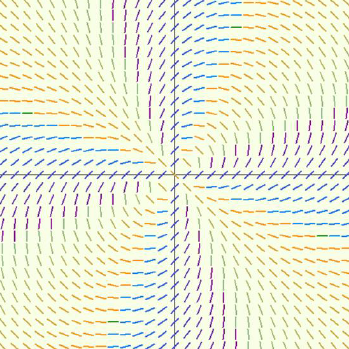
\includegraphics[scale = 0.5]{1.png}}
        \end{center}
    \end{tcolorbox}

\newpage
\textbf{Differenciálegyenletek II:}    

    \begin{tcolorbox}[colback=red!5!white,colframe=red!60!black,title= 1. Szeparábilis és arra visszavezethető DE]
        \textbf{Definíció:} \\
        Az olyan $y' = f(x,y)$ elsőrendű DE-et, amely $y' = h(x) \cdot g(y)$ alakra hozható, szeparábilis (változóiban szétválasztható) differenciálegyenletnek nevezzük. Feltesszük, hogy $h$ és $g$ valamely, alkalmas $I$ és $J$ intervallumon folytonosak. \\
        \textbf{Megoldás:} \\
        $$\dfrac{dy}{dx} = y' = h(x) \cdot g(y)$$
        $$\int\dfrac{1}{g(y)}dy = \int h(x)dx$$
        \textbf{Szinguláris megoldás:} $g(y) = 0$, amivel osztani kell \\
        \textbf{Nem szinguláris megoldás:} $g(y) \neq 0$ \\
        Szeparábilis differenciálegyenletre visszavezethetőek más DE-ek is $u$ helyettesítéssel:
        $$y' = f(ax + by + c)$$
        $$u := ax + by + c$$
        $$u' = \dfrac{du}{dx} = a + by' = a + b \cdot f(u)$$
        illetve
        $$y' = f(1,\dfrac{y}{x})$$
        $$u = \dfrac{y}{x}$$
        $$u' = \dfrac{du}{dx} = \dfrac{y'x - y \cdot 1}{x^2} = \dfrac{y'}{x} - \dfrac{y}{x^2} = \dfrac{y' - \dfrac{y}{x}}{x}$$
        Továbbá, fontos még az is, hogy az elsőrendű, lineáris differenciálegyenleteknek a homogén része is szétválasztható DE-re vezethető vissza.
    \end{tcolorbox}

    \begin{tcolorbox}[colback=red!5!white,colframe=red!60!black,title= 2. Bernoulli-féle DE]
       \textbf{Definíció:} \\
       Az $y' + p(x) \cdot y = q(x) \cdot y^n (n \neq 0, n \neq 1)$ alakú, elsőrendű, nemlineáris DE-et. Bernoulli-féle differenciálegyenletnek nevezzük, ahol $p, q: I \subset \mathbb{R} \rightarrow \mathbb{R}$ folytonos függvények. \\
       \textbf{Megoldás helyettesítéssel:} \\
       $$z(x) = z = y^{1-n} \quad\quad \text{(eredeti DE)}$$
       $$z' = \dfrac{dz}{dx} = (1-n) \cdot y^{-n} \cdot y' \quad\quad (1)$$
       Ahonnan az eredeti DE-et $y^n$-nel leosztva, a (1) egyenletet pedig $1-n$-nel leosztva és felhasználva a helyettesítést, azt kapjuk, hogy:
       $$\dots$$
    \end{tcolorbox}
\end{document}